\documentclass[12pt]{article}
% Margin definition.
\usepackage[a4paper,total={6.8in, 8.5in}]{geometry}
\usepackage{parskip}
\usepackage[bottom]{footmisc}
% Images.
\usepackage{graphicx}
\graphicspath{{images/}}
\usepackage[export]{adjustbox}
\usepackage{float}
% Table
\usepackage{array}
\usepackage[toc,page]{appendix}
% Links.
\usepackage[T1,hyphens]{url}
\usepackage[hidelinks, bookmarks=true]{hyperref}
% Encoding.
\usepackage[utf8]{inputenc}
% Header for ua logo.
\usepackage{fancyhdr}
% Hedear with ua logo definition. 
\pagestyle{fancy}
\fancyhf{}
\chead{
    
\includegraphics[scale=0.2]{logo_UA.png}
}
\setlength\headheight{45pt}
% Footer with page number.
\rfoot{Page \thepage}
\renewcommand{\footrulewidth}{0.4pt}
% Rename table of contents title to "Index"
\renewcommand{\contentsname}{Index \vspace{0.2cm}}

\begin{document}

\title{\vspace{-0.9cm}
       \Large\raggedright\textbf{Software Quality and Tests} \\ 
       \large\raggedright\textbf{Homework 1 : Test Development} \\ 
       \vspace{0.5cm}
       \normalsize
       \raggedright\textbf{Author: \hspace{1.1cm} André Pedrosa} \\ \vspace{0.1cm}
       \raggedright\textbf{N. Mec.: \hspace{0.92cm} 85098} \\ \vspace{0.1cm}
       \raggedright\textbf{Date: \hspace{1.6cm} 06/05/2019} \\ \vspace{0.1cm}
       \raggedright\textbf{Repository: \hspace{0.35cm} \url{https://github.com/aspedrosa/weather\_forecast/}} \\}
\date{} %This way the date from the maketitle command doesn't appear

\maketitle
\thispagestyle{fancy}

\vspace{-1.4cm}

\tableofcontents

\newpage

\section{Intro}

This homework consisted in developing a web project that allows to see the
  meteorology state for the next days, for a specific location, with the main goal
  being to develop the different classes of tests (unitary, integration and functional)
  along with the development of the project.

The main components of the solution are:
\begin{itemize}
  \item \textbf{Web page}, allowing the user to select and search for locations and also giving
    the choice to the user to choose how many days of forecast data he wants to see.
  \item \textbf{Rest API}, that can be called by external clients allowing to query the
    meteorology state for a specific location.
  \item \textbf{Integration with an external source}, from where the real meteorologic data will be
    obtained, so the app built is a client of another source.
  \item \textbf{Caching mechanism}, where is stored the last retrieved results from recent calls to the
    external sources, having also some statistics about its functioning (number of requests,
    hits and misses)
\end{itemize}

For the website jQuery and Bootstrap was used. To implement the server side logic a web
  application was built using SpringBoot.

\section{Solution}
\subsection{Front End}

The front end consists on a single minimalist page, where the user can do every thing
  that the system allows on one page.

At the start the user can either search from a specific location or use the "I'm Feeling Lucky"
  feature where the meteorology state for the first location found on the results of
  the search mechanism is displayed. At this time the user also can choose how much days
  of meteorologic data he wants to see.

\begin{figure}[h]
  \center
  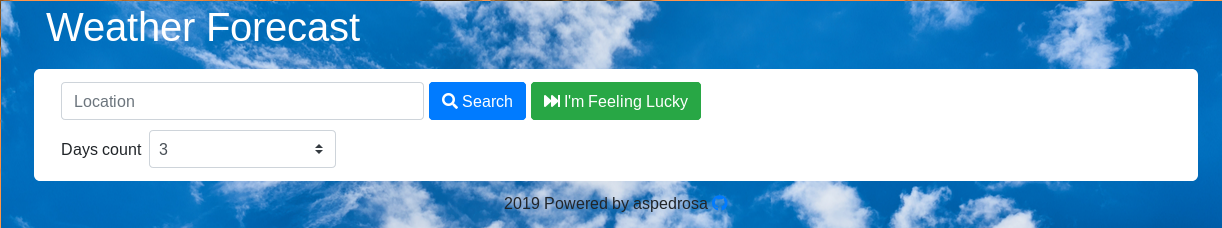
\includegraphics[scale=0.35]{start_website.png}
  \caption{How the web page is displayed at the beginning}
\end{figure}

Once the user searches for a location, a table appears with the names of related location
  as well as the respective geographic coordinates.

\begin{figure}[h]
  \center
  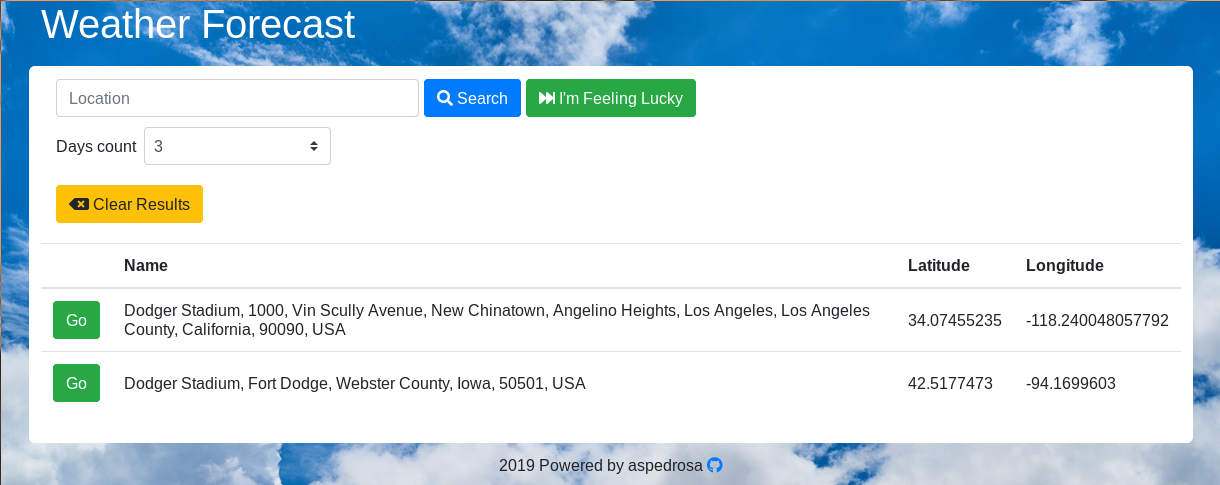
\includegraphics[scale=0.35]{after_search_website.png}
  \caption{Search results for "dodger stadium"}
\end{figure}

When the user chooses a location two types of forecast data is displayed. Current and for
  future days, being the number of days the same as the value on the "Days Count" select html tag.

\begin{figure}[h]
  \center
  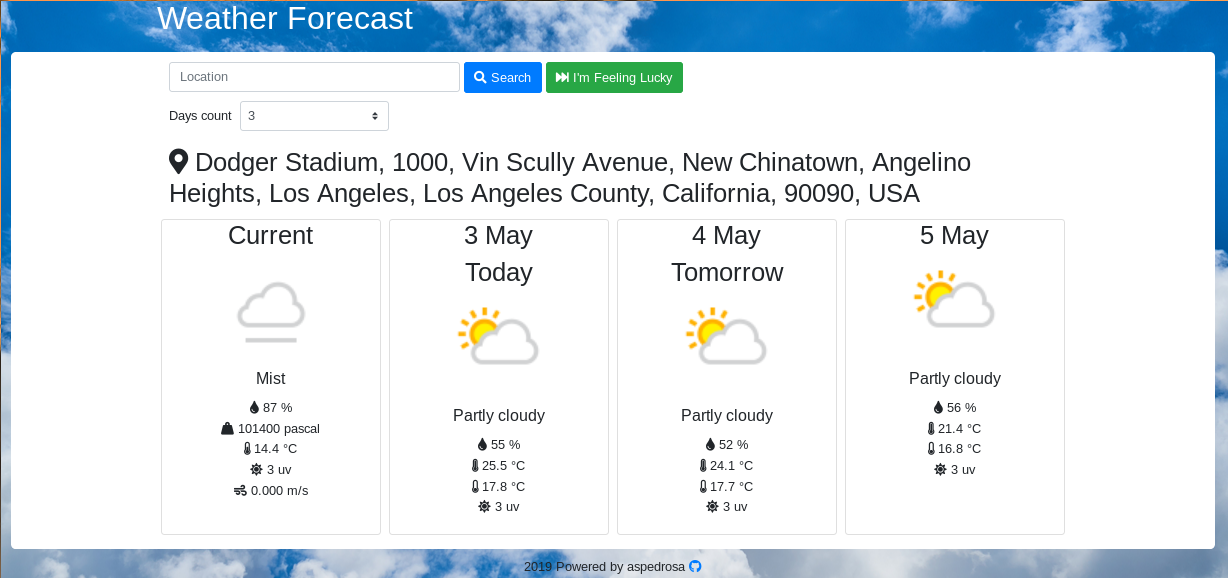
\includegraphics[scale=0.35]{forecast_data_website.png}
  \caption{Forecast data for "Dodger Stadium, California, USA"}
\end{figure}

\subsection{Back End}

\begin{figure}[h]
  \center
  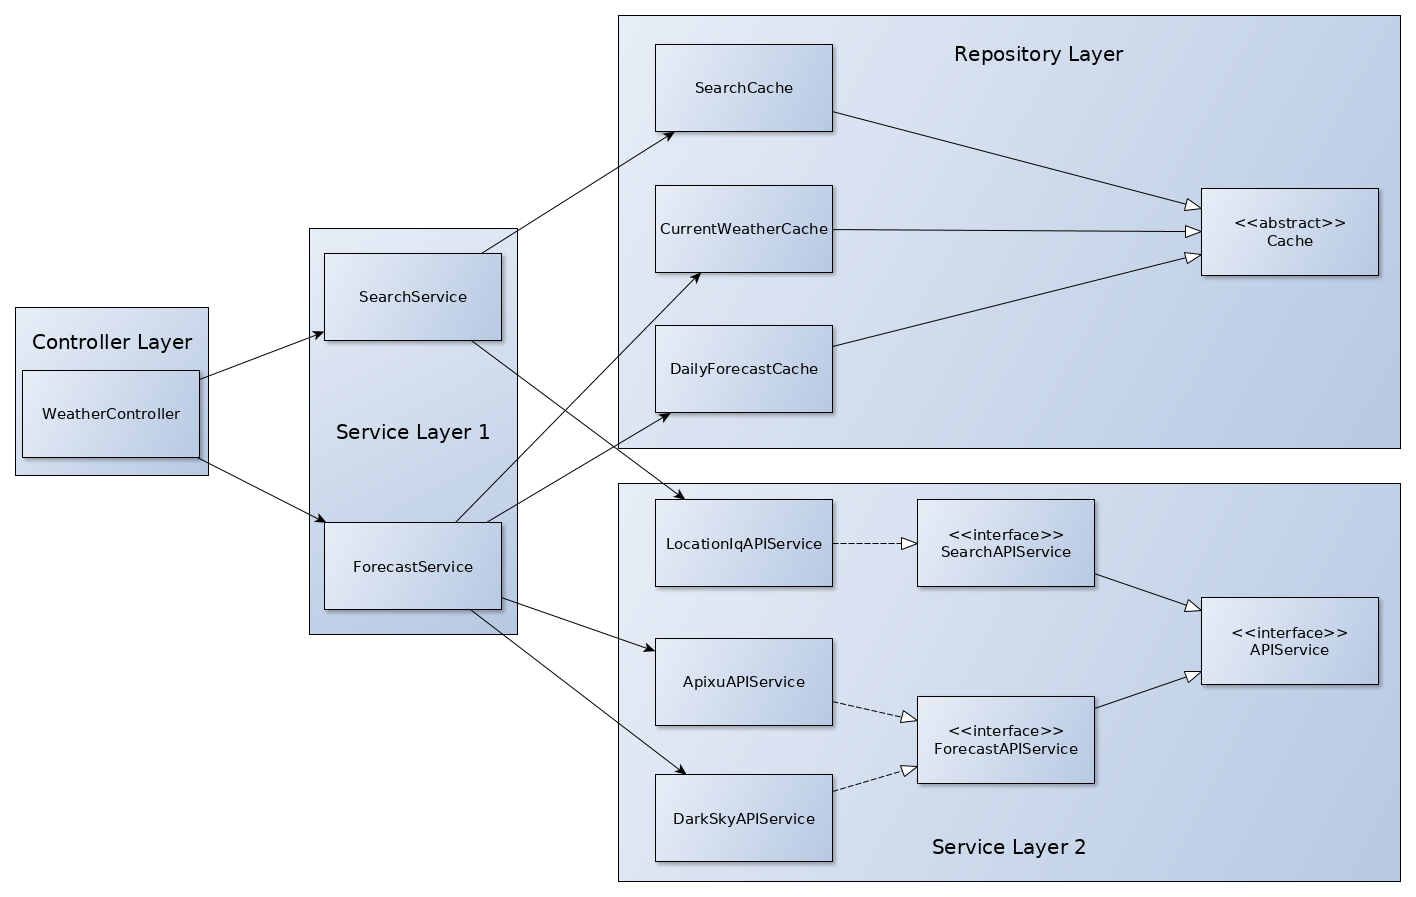
\includegraphics[scale=0.35]{solution.png}
  \caption{Class diagram for the solution implemented}
  \label{fig_class_diagram}
\end{figure}

As mentioned before, back end uses SpringBoot, that divides the system in three layers. Controllers,
  that process HTTP requests and pass the received data to the service layer. The service layer
  imposes the business logic. The last layer is the repositories where the service layers can store
  data.

On figure \ref{fig_class_diagram} is shown the several layers of the application as well as the
  classes in each one. Abstraction where used to allow extensibility to the application such as
  caching new types of data, using other external apis and using other external apis for new
  types of data.

\subsubsection{Controller}

The controller layer is composed by a single controller where the REST API is
  defined. Has two paths:
  \begin{itemize}
    \item api/forecast : Obtains meteorologic data of a location
      \begin{itemize}
        \item latitude : double : request parameter - mandatory : latitude of the location
        \item longitude : double : request parameter - mandatory : longitude of the location
        \item days\_count : int : request parameter : how much days of forecast data to retrieve
      \end{itemize}
    \item api/search : searches for a location. Used to obtain geographic coordinates
      \begin{itemize}
        \item location : String : request parameter - mandatory : location to search for.
      \end{itemize}
    %\item api/cache\_stats
  \end{itemize}

The controller is also responsible to validate to parameters received before sending them to the
  first service layer (i.e. latitude must be a double).

\subsubsection{Services}

Is composed by the upper layer (Service Layer 1) and the lower layer (Service Layer 2). The upper layers
  is used by the WeatherController class and its role is to check the cache for the requested data and if
  it is not there should interact with the lower layer. The role of the lower layer is to retrieve
  meteorologic from the external api. Whenever the upper layer contacts the lower layer to
  get data it must store that received data in the cache.

The upper layer is composed by two services, Search and Forecast. Both follow the flow mentioned
  previously, however the Forecast service as a complexer logic to when query the lower layer. First
  the Forecast service is in charge of two types of data, current and daily forecast, leading to
  two caches with different expiration times. Secondly the Forecast service uses two services
  of the lower layer. One used as a primary and other as backup in case the primary fails. Furthermore,
  if the client asks for a high number of days of forecast data, the Forecast service tries to use the
  one that offers the higrer number of days of forecast data.

\begin{figure}[h]
  \center
  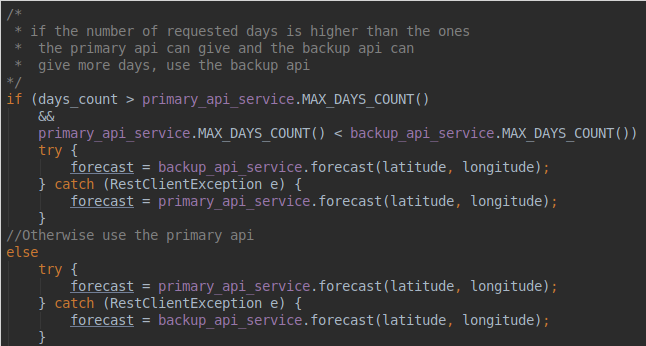
\includegraphics[scale=0.5]{primary_backup_apis.png}
  \caption{Block of code of the function retrieve\_from\_apis of the class ForecastService where
    the choice of which api to use happens}
\end{figure}

  Third both current and daily data are retrieved on one call to an external api. So, if the
  current data expires, both current and daily data will be stored in cache after the call
  and overwriting of existing data may occur but because the new data is more recent, is more
  accurate, so overwriting ends up being a good thing.

\subsubsection{Repositories}

The repository layer is in charge implementing caching mechanisms for the application. This is done
  associating data to a key, in other words, a map was used. Each cached data has a time-to-live
  after which the data stored is not valid and if clients asks for that data, should consider as not
  not having that data cached.

Different types of data have different strategies to see if it had expired. For current meteorologic data
  and search data is just checking, whenever its requested, if a certain time has passed since the
  last write (30 days for search data, because location data it's pretty stable and 15 min for
  current meteorologic data). In this cases the data associated is just removed if its considered as
  expired. For daily forecast all data isn't removed since daily forecast data can be associated
  with several days, witch means is a list of values each position associated with a different day. So the data
  "expires" when the current date is in a different date comparing to the date on the last write (i.e. if
  data is stored at 12/05/2019 10:00, at 12/05/2019 15:00 is still valid but at 13/05/2019 10:00 isn't).
  When this happens the data needs to be shifted the difference of days since of last write, however if
  the number of days that had passed is higher than the number of days stored than the data is just removed.

\begin{figure}[h]
  \center
  \includegraphics[scale=1.5]{expiration.png}
  \caption{Difference of cache strategies between current weather and search and daily forecast.
    The two methods here shown are called whenever the cache is queried for data. If the
    method has\_value\_expired returns true then the method handle\_expired\_value is called. On the method
    get\_cached\_data of the class Cache its clear what happens when the system tries to get
    cached data.}
\end{figure}

\section{Tests}

As said in the Intro, the main goal of this homework is to develop a project with
  test development along. On this section it is explained what tests were made
  and how they were made.

\subsection{Front End}

Here functional tests were made that validate the functional requirements for the application such as:
\begin{itemize}
  \item give an error if the user inserts an unknown location
  \item the number of days of forecast data displayed must be the same as the number
    of days requested
  \item give an error if the user insert an invalid location
  \item when the user uses the I'm Feeling Lucky feature, the forecast data should be
    displayed, without asking to choose a location
\end{itemize}

Because this the web page uses the api developed, its response to the web page
  was mocked with deterministic responses using Mockito.

\subsection{Back End}
\subsubsection{Controller}

Here is tested the responsibilities of the controllers:
\begin{itemize}
  \item generate the response accordingly to the response received from the service layer
  \item validation of the parameters received
\end{itemize}
The integration tests for controllers were done by mocking the service layers and the application
  context is restricted to Model-View-Controller(MVC) components.

\subsubsection{Services}

For integration tests of the upper layer the lower layer services and repositories were mocked allowing
  to test:
\begin{itemize}
  \item ForecastService
    \begin{itemize}
      \item usage of the cache
      \item query external api when one of the cache doesn't satisfies the request (i.e.
        number of days requested is higher than the days stored or no current data
        cached)
      \item choice between the primary and backup api according to number of days requested
      \item choice between the primary and backup api according to availability
    \end{itemize}
  \item SearchService
    \begin{itemize}
      \item successful responses
      \item not found location
    \end{itemize}
\end{itemize}

For the lower layer only unitests were made mocking the response of the external api. For the
  services that implement the interface ForecastAPIService (DarkSkyAPIService and
  ApixuAPIService) it was tested:
  \begin{itemize}
    \item the conversion of weather metrics to si units
    \item number of days processed and generated had to be the same as the number of days
      received from the external api
  \end{itemize}
  For the services that implement the SearchAPIService (LocationIqAPIService) it was tested:
  \begin{itemize}
    \item handle the user inserting an unknown location leading to no results
    \item handle receiving multiple entries with the same name from the external api
  \end{itemize}

\subsubsection{Repositories}

To test the layer of repositories only units were done. Because the class SearchCache and
  CurrentWeatherCache only change the time-to-live comparing to their super class, these classes were not tested however
  their super class, abstract, was tested by creating a new implementation during the tests with a low
  time-to-live making tests doable:
  \begin{itemize}
    \item receiving null after time-to-live
    \item receive data after insert
    \item not receiving data if no inserted were made
    \item overwrite and update of data updates write date
  \end{itemize}
  For some of these tests an external library(Awaitility) was used that allows to verify a condition
    during a certain time. If at the end of that time the condition is not met,
    the test fails. At first the Thread.sleep method was used but Sonarcloud didn't
    recommended that method.

Because the DailyForecastCache has different ways to handle data expiration and
  the expiration itself is different separate tests were done for:
  \begin{itemize}
    \item expired data is correctly handled
    \item data expires on the correct time
    \item the action of overriding data is done correctly
  \end{itemize}
  To test the expiration of the data an external library (joda-time) was used to allow
    control of time. Basically whenever the current time is needed on the application this
    a function from this library is used to allow control of time during tests.

\section{Sonarcloud}


For static code analysis I used Sonarcloud (\url{https://sonarcloud.io/dashboard?id=aspedrosa\_weather\_forecast}).

\begin{figure}[h]
  \center
  \includegraphics[scale=1.5]{sonarcloud.png}
\end{figure}

Currently, the project has 93.7\% code coverage and 30 unit tests. 77 code smells
  are present because sonarcloud uses a different naming convention (camel case) from the one used
  (snake case).

The 2 duplicated blocks are present on the parsing of the response from
  the external apis. Both use setters of the classes DailyForecast and CurrentWeather
  to build the response for higher layers but the two external apis used have different
  response structure making it hard and not code friendly to eliminate these duplicated
  blocks.

The 6 security hotstops concern security problems that can exists. The problems that
  were mentioned were related to user input such as command line arguments (not used), HTTP arguments
  (in case of the /api/forecast path, request parameters are checked against a regex) and
  using regex for user input check (sonarcloud warns that for complicated regexs, the verification can
  take a lot of cpu load, however the regexs used are basic and don't have heavy recursions such
  as \textit{(a+)+}).

\end{document}
